\documentclass{beamer}
\usepackage{ragged2e}
\usepackage{CJKutf8}
\usepackage{tikz}
\setbeamertemplate{theorems}[numbered]
\justifying\let\raggedright\justifying
\begin{document}
\begin{CJK*}{UTF8}{gbsn}

\newtheorem{Thm}{定理}[section]
\theoremstyle{definition}
\newtheorem{Def}{定义}[section]
\theoremstyle{example}
\newtheorem*{Ex}{例:}
\newtheorem{Exercise}{习题}
\newtheorem{Exercise1}{习题}

\date{}
\author{陈建文}

\title{第一章 集合及其运算}
\begin{frame}
  \titlepage
\end{frame}  
\section{集合的概念}
\begin{frame}
  \frametitle{1. 集合的概念}
  \begin{Def}
    通常把一些互不相同的东西放在一起所形成的整体叫做一个\alert{集合}。构成集合的每个东西叫做集合的\alert{元素}。
给定一个集合$A$和一个元素$a$,用\alert{$a \in A$}表示$a$是$A$的一个元素,用\alert{$a \notin A$}表示$a$不是$A$的一个元素。
  \end{Def}
\end{frame}

\begin{frame}
  \frametitle{1. 集合的概念}

有两种方法表示一个集合:
\begin{enumerate}
\item 把构成集合的那些元素全部列出来
  \begin{itemize}
\pause
  \item $A = \{1, 2, 3\}$
\pause
\item $C = \{a, b, c, \ldots, z\}$
  \end{itemize}
\pause
\item 用概括集合中各元素的属性来表示集合$\{x|P(x)\}$
\begin{itemize}
\pause
\item $E = \{n|n \in \mathcal{Z} \land n\text{ is even}\}$
\pause
\item $E = \{n \in \mathcal{Z} | n\text{ is even}\}$
\end{itemize}
\end{enumerate}


\end{frame}

\begin{frame}
  \frametitle{1. 集合的概念}
  \begin{tabular}{cc|c}
    p& q& p $\land$ q\\
    \hline
    T&T&T\\
    T&F&F\\
    F&T&F\\
    F&F&F\\
  \end{tabular}\hspace{1cm}
  \begin{tabular}{cc|c}
    p& q& p $\lor$ q\\
    \hline
    T&T&T\\
    T&F&T\\
    F&T&T\\
    F&F&F\\
  \end{tabular}\hspace{1cm}
  \begin{tabular}{c|c}
    p& $\lnot$ p\\
    \hline
    T&F\\
    F&T\\
  \end{tabular}

    \begin{tabular}{cc|c}
    p& q& p $\to$ q\\
    \hline
    T&T&T\\
    T&F&F\\
    F&T&T\\
    F&F&T\\
  \end{tabular}\hspace{0.87cm}
  \begin{tabular}{cc|c}
    p& q& p $\leftrightarrow$ q\\
    \hline
    T&T&T\\
    T&F&F\\
    F&T&F\\
    F&F&T\\
  \end{tabular}
\end{frame}

\begin{frame}
  \frametitle{1. 集合的概念}

存在一个集合,该集合中不包含任何元素,称为\alert{空集},记为$\Phi$。

\end{frame}

\section{子集、集合的相等}
\begin{frame}
  \frametitle{2. 子集、集合的相等}

  \begin{Def}
    设$A$,$B$为两个集合,如果$A$中的每个元素都是$B$中的元素,并且$B$中的每个元素都是$A$中的元素,则称$A$与$B$\alert{相等},并记为\\ $A=B$。
  \end{Def}
  \begin{itemize}
\pause
  \item   $\{1,2,3,4,5\} = \{3,4,2,1,5\}$
\pause
\item $\{x \in \mathcal{R} | x^2 -5x + 6 = 0\} = \{2,3\}$
  \end{itemize}
\end{frame}
\begin{frame}
  \frametitle{2. 子集、集合的相等}
  \begin{Def}
设$A$,$B$为两个集合,如果$A$中的每个元素都是$B$中的元素,则称$A$为$B$的
\alert{子集},记为$A \subseteq B$; 如果$A \subseteq B$并且$A \neq B$,则称 $A$为$B$ 的\alert{真子集},记为$A\subset B$。    
  \end{Def}
  \begin{itemize}
\pause
  \item   $\{1,2,4\} \subseteq \{1,2,3,4,5\}$
\pause
\item $\{1,2,4\} \subset \{1,2,3,4,5\}$
  \end{itemize}
\end{frame}
\begin{frame}
  \frametitle{2. 子集、集合的相等}
  \begin{Thm}
   空集是任一个集合的子集且空集是唯一的。 
  \end{Thm}
\end{frame}
\begin{frame}
  \frametitle{2. 子集、集合的相等}

\begin{Def}
  集合$S$的所有子集构成的集合称为$S$的幂集,记为$2^S$或者$\mathcal{P}(S)$。
\end{Def}\pause
\begin{Ex}
  设$S=\{1,2,3\}$,则$2^s=\{\phi, \{1\},\{2\},\{3\},\{1,2\},\{1,3\},\{2,3\},\{1,2,3\}\}$。
\end{Ex}
\end{frame}
\section{集合的基本运算}
\begin{frame}
  \frametitle{3. 集合的基本运算}
\begin{minipage}{0.69\linewidth}
  \begin{Def}
    设$A,B$为任意的两个集合,至少属于集合 $A$ 与集合$B$之一的那些元素构成的集合称为 $A$ 与 $B$的\alert{并集},记为$A \cup B$。
    \begin{equation*}
      A\cup B = \{x|x \in A \lor x \in B\}
    \end{equation*}
  \end{Def}\pause
\end{minipage}
\begin{minipage}{0.29\linewidth}
%    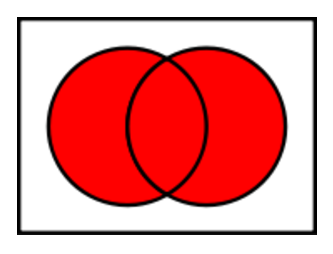
\includegraphics[width=2.5cm,height=2cm]{union}
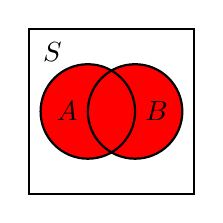
\begin{tikzpicture}[thick, scale=0.3]
  \draw (-3.5, -3.5) rectangle (3.5, 3.5);
  \filldraw[fill=red] (-1,0) circle [radius=2cm]
               (1,0) circle [radius=2cm];
  \draw (-1,0) node[left] {$A$};
  \draw (1,0) node[right] {$B$};
  \draw (-2.5,2.5) node {$S$};
\end{tikzpicture}
  \end{minipage}\pause
    \begin{Ex}
        $\{1,2\} \cup \{2,3\} = \{1,2,3\}$
    \end{Ex}
\end{frame}
\begin{frame}
  \frametitle{3. 集合的基本运算}
\begin{minipage}{0.69\linewidth}
  \begin{Def}
    设$A,B$为任意的两个集合,由既属于集合 $A$ 又属于集合$B$的所有元素构成的集合称为 $A$ 与 $B$的\alert{交集},记为$A \cap B$。
    \begin{equation*}
      A\cap B = \{x|x \in A \land x \in B\}
    \end{equation*}
  \end{Def}\pause
\end{minipage}
\begin{minipage}{0.29\linewidth}
%    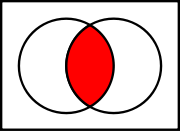
\includegraphics[width=2.5cm,height=2cm]{intersection}
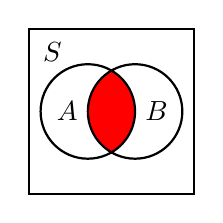
\begin{tikzpicture}[thick, scale=0.3]
  \draw (-3.5, -3.5) rectangle (3.5, 3.5);
  \fill[red] (-0.01, 0 |- -60:2cm) arc [start angle=-60, end angle = 60, radius = 2cm];
  \fill[red] (0.01, 0 |- 120:2cm) arc [start angle=120, end angle = 240, radius = 2cm];
  \draw (-1,0) circle [radius=2cm]
               (1,0) circle [radius=2cm];
  \draw (-1,0) node[left] {$A$};
  \draw (1,0) node[right] {$B$};
  \draw (-2.5,2.5) node {$S$};
\end{tikzpicture}
  \end{minipage}\pause
    \begin{Ex}
        $\{1,2\} \cap \{2,3\} = \{2\}$
    \end{Ex}
\end{frame}
\begin{frame}
  \frametitle{3. 集合的基本运算}
\begin{minipage}{0.69\linewidth}
  \begin{Def}
    设$A,B$为任意的两个集合,由属于集合$A$但不属于集合$B$的所有元素构成的集合称为 $A$ 与 $B$的\alert{差集},记为$A \setminus B$。
    \begin{equation*}
      A\setminus B = \{x|x \in A \land x \notin B\}
    \end{equation*}
  \end{Def}\pause
\end{minipage}
\begin{minipage}{0.29\linewidth}
%    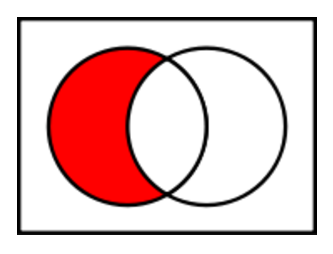
\includegraphics[width=2.5cm,height=2cm]{relative}
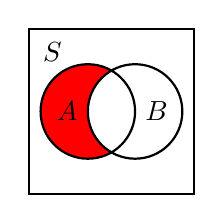
\begin{tikzpicture}[thick, scale=0.3]
  \draw (-3.5, -3.5) rectangle (3.5, 3.5);
\fill[red] (0,0 |- 60:2cm) arc [start angle=60, end angle = 300, radius = 2cm]
                           arc [start angle=240, end angle = 120, radius = 2cm];
  \draw (-1,0) circle [radius=2cm]
               (1,0) circle [radius=2cm];
  \draw (-1,0) node[left] {$A$};
  \draw (1,0) node[right] {$B$};
  \draw (-2.5,2.5) node {$S$};
\end{tikzpicture}
  \end{minipage}\pause
    \begin{Ex}
        $\{1,2\} \setminus \{2,3\} = \{1\}$
    \end{Ex}
\end{frame}
\begin{frame}
  \frametitle{3. 集合的基本运算}
\begin{minipage}{0.69\linewidth}
  \begin{Def}
    在许多实际问题中,常以某个集合$S$为出发点,而所涉及的集合都是$S$的子集。这个包含所考虑的所有集合的集合$S$,称为该问题的\alert{全集}。如果$A$是$S$的子集,则差集$S \setminus A$称为集合$A$对集合$S$的\alert{余集},记为$A^c$。
    \begin{equation*}
      A^c = \{x|x \in S \land x \notin A\}
    \end{equation*}
  \end{Def}\pause
\end{minipage}
\begin{minipage}{0.29\linewidth}
%    \includegraphics[width=2.5cm,height=2cm]{absolute}
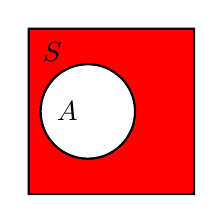
\begin{tikzpicture}[thick, scale=0.3]
  \filldraw[fill=red] (-3.5, -3.5) rectangle (3.5, 3.5)
               (-1, 0) circle [radius = 2cm];
  \draw (-1,0) node[left] {$A$};
  \draw (-2.5,2.5) node {$S$};
\end{tikzpicture}
  \end{minipage}\pause
    \begin{Ex}
        $S = \{0,1\}, A =  \{0\},$ 则$A^c = \{1\}$
    \end{Ex}
\end{frame}


\begin{frame}
  \frametitle{3. 集合的基本运算}
  \begin{Thm}
设$S$为全集,$\emptyset$为空集,$A$,$B$,$C$为$S$的子集,则\\
1. $A \cup B = B \cup A$, $A \cap B = B \cap A$.\\
2. $(A \cup B) \cup C = A \cup (B \cup C)$,$(A \cap B) \cap C = A \cap (B \cap C)$.\\
%3. $A \cup A = A$,$A \cap A = A$.\\
%4. $(A \cup B) \cap A = A$,$(A \cap B) \cup A = A$.\\
4. $A \cup \emptyset = A$, $A \cap \emptyset = \emptyset$.\\
5. $A \cup S = S$, $A \cap S = A$.\\
6. $A \cap (B \cup C) = (A \cap B) \cup (A \cap C)$, $A \cup (B \cap C) = (A \cup B) \cap (A \cup C)$.\\
7. $A \cup A^c = S$, $A \cap A^c = \emptyset$.\\
8. $C\setminus (A \cup B) = (C \setminus A) \cap (C \setminus B)$, $C \setminus (A \cap B) = (C \setminus A) \cup (C \setminus B)$.\\ 
8'. $(A \cup B)^c = A^c \cap B^c$, $(A \cap B)^c = A^c \cup B^c$.\\
  \end{Thm}
\end{frame}

% \begin{frame}
%   \frametitle{3. 集合的基本运算}
%   \begin{tabular}{cc|c}
%     p& q& p $\land$ q\\
%     \hline
%     T&T&T\\
%     T&F&F\\
%     F&T&F\\
%     F&F&F\\
%   \end{tabular}\hspace{1cm}
%   \begin{tabular}{cc|c}
%     p& q& p $\lor$ q\\
%     \hline
%     T&T&T\\
%     T&F&T\\
%     F&T&T\\
%     F&F&F\\
%   \end{tabular}\hspace{1cm}
%   \begin{tabular}{c|c}
%     p& $\lnot$ p\\
%     \hline
%     T&F\\
%     F&T\\
%   \end{tabular}

%   \vspace{1cm}\pause
%     \begin{tabular}{cc|c}
%     x& y& x $\land$ y\\
%     \hline
%     1&1&1\\
%     1&0&0\\
%     0&1&0\\
%     0&0&0\\
%   \end{tabular}\hspace{1cm}
%   \begin{tabular}{cc|c}
%     x& y& x $\lor$ y\\
%     \hline
%     1&1&1\\
%     1&0&1\\
%     0&1&1\\
%     0&0&0\\
%   \end{tabular}\hspace{1cm}
%   \begin{tabular}{c|c}
%     x& $\bar{x}$\\
%     \hline
%     1&0\\
%     0&1\\
%   \end{tabular}

% \end{frame}
% \begin{frame}
%   \frametitle{3. 集合的基本运算}
%   \begin{Def}
%     设$B$是一个集合,在其上定义了一个一元运算 $\ \bar{}\ $,两个二元运算$\lor$和$\land$,以及两个特定的元素$0$和$1$,使得对$B$中的任何元素$x$,$y$,$z$,满足以下条件,则称$(B, \ \bar{}\ , \lor, \land, 0, 1)$为一个\alert{布尔代数}。
%     \begin{align*}
%       1. &x \lor y = y \lor x, x \land y = y \land x\\
%       2. &(x \lor y) \lor z = x \lor (y \lor z), (x \land y) \land z = x \land (y \land z) \\
%       3. &x \lor 0 = x \\
%       4. &x \land 1 = x \\
%       5.&x \lor (y \land z) = (x \lor y) \land (x \lor z), x \land (y \lor z) = (x \land y) \lor (x \land z)\\
%       6. &x \lor \bar{x} = 1, x \land \bar{x} = 0\\
%     \end{align*}
%   \end{Def}
% \end{frame}
\begin{frame}
  \frametitle{3. 集合的基本运算}
\begin{minipage}{0.69\linewidth}
  \begin{Def}
    设$A,B$为两个集合,$A\setminus B$与$B\setminus A$的并集称为$A$与$B$的\alert{对 称 差},记为$A \bigtriangleup B$。
    \begin{equation*}
      A\bigtriangleup B = (A \setminus B) \cup (B \setminus A)
    \end{equation*}
  \end{Def}\pause
\end{minipage}
\begin{minipage}{0.29\linewidth}
%    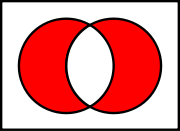
\includegraphics[width=2.5cm,height=2cm]{symmetric}
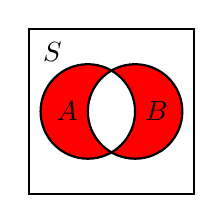
\begin{tikzpicture}[thick, scale=0.3]
  \draw (-3.5, -3.5) rectangle (3.5, 3.5);
\fill[red] (0,0 |- 60:2cm) arc [start angle=60, end angle = 300, radius = 2cm]
                           arc [start angle=240, end angle = 120, radius = 2cm];
\fill[red] (0,0 |- 60:2cm) arc [start angle=120, end angle = -120, radius = 2cm]
                           arc [start angle=-60, end angle = 60, radius = 2cm];
  \draw (-1,0) circle [radius=2cm]
               (1,0) circle [radius=2cm];
  \draw (-1,0) node[left] {$A$};
  \draw (1,0) node[right] {$B$};
  \draw (-2.5,2.5) node {$S$};
\end{tikzpicture}
  \end{minipage}\pause
    \begin{Ex}
        $\{1,2\} \bigtriangleup \{2,3\} = \{1,3\}$
      \end{Ex}
      \pause
      \begin{Thm}
        设$S$为全集,$A\in 2^S$,$B\in 2^S$,则
        \begin{equation*}
          A \bigtriangleup B = (A \cap B^c)\cup (A^c \cap B)
        \end{equation*}
      \end{Thm}
\end{frame}

\begin{frame}
  \frametitle{3. 集合的基本运算}
  \begin{Thm}
设$S$为全集,$\emptyset$为空集,$A$,$B$,$C$为$S$的子集,则\\
1. $A \bigtriangleup B = B \bigtriangleup A$.\\
2. $(A \bigtriangleup B) \bigtriangleup C = A \bigtriangleup (B \bigtriangleup C)$.\\
3. $\emptyset \bigtriangleup A = A$.\\
4. $A \bigtriangleup A = \emptyset$.\\
5. $A \cap (B \bigtriangleup C) = (A \cap B) \bigtriangleup (A \cap C)$.\\ 
  \end{Thm}
\end{frame}

% \begin{frame}
%   \frametitle{3. 集合的基本运算}
%   \begin{tabular}{cc|c}
%     p& q& p $\oplus$ q\\
%     \hline
%     T&T&F\\
%     T&F&T\\
%     F&T&T\\
%     F&F&F\\
%   \end{tabular}

%   \vspace{1cm}\pause
%     \begin{tabular}{cc|c}
%     x& y& x $\oplus$ y\\
%     \hline
%     1&1&0\\
%     1&0&1\\
%     0&1&1\\
%     0&0&0\\
%     \end{tabular}
% \end{frame}

% \begin{frame}
%   \frametitle{3. 集合的基本运算}
%   \begin{Def}
%     设$(B, \ \bar{}\ , \lor, \land, 0, 1)$为一个布尔代数,$x \in B, y \in B$,定义 $x$与$y$的\alert{对称差}为
%     $x \oplus y = (x \land \bar{y}) \lor (\bar{x} \land y)$。
%   \end{Def}
%   \begin{Thm}
%     设$(B, \ \bar{}\ , \lor, \land, 0, 1)$为一个布尔代数,$x \in B, y \in B, z \in B$。则\\
% 1. $x \oplus y = y \oplus x$.\\
% 2. $(x \oplus y) \oplus z = x \oplus (y \oplus z)$.\\
% 3. $0 \oplus x = x$.\\
% 4. $x \oplus x = 0$.\\
% 5. $x \land (y \oplus z) = (x \land y) \oplus (x \land z)$.\\ 
%   \end{Thm}
% \end{frame}

\begin{frame}
  \frametitle{3. 集合的基本运算}
  \begin{Def}  \justifying\let\raggedright\justifying
    以集合为元素的集合称为\alert{集族}。如果$I$为任意一个集合,对$I$中每个元素$\alpha$都有一个唯一的集合与之对应,这个集合记为$A_{\alpha}$,那么所有这些$A_{\alpha}$形成的集族可以用$\{A_{\alpha}\}_{\alpha \in I}$表示,其中$I$称为\alert{标号集}。
  \end{Def}
  \begin{Def}
    集族$\{A_{\alpha}\}_{\alpha \in I}$中所有集合的并集$\bigcup_{\alpha \in I}A_{\alpha}$定义为
\[ \bigcup_{\alpha \in I}A_{\alpha} = \{x|\exists \alpha \in I \text{使得} x \in A_{\alpha}\}\]
    集族$\{A_{\alpha}\}_{\alpha \in I}$中所有集合的交集$\bigcap_{\alpha \in I}A_{\alpha}$定义为
\[ \bigcap_{\alpha \in I}A_{\alpha} = \{x|\forall \alpha \in I, x \in A_{\alpha}\}\]
  \end{Def}
\end{frame}

\begin{frame}
  \frametitle{3. 集合的基本运算}
  \begin{Ex}
    设$I=\{x \in \mathbb{R} | 0 < x \leq 1\}$,$\forall x \in \mathbb{R}, A_x=\{y\in \mathbb{R}|0 < y < x\}$,
    则
    \begin{equation*}
      \bigcup_{x\in I}A_x=?,
      \bigcap_{x\in I}A_x=?      
    \end{equation*}
  \end{Ex}
\end{frame}

\begin{frame}
  \frametitle{3. 集合的基本运算}
\begin{Thm}
设$A$为任意集合, $\{B_{\alpha}\}_{\alpha \in I}$为任意一个集族,则
\begin{enumerate}
\item $A \cap (\bigcup_{\alpha \in I}B_{\alpha}) = \bigcup_{\alpha \in I}(A \cap B_{\alpha})$
\item $A \cup (\bigcap_{\alpha \in I}B_{\alpha}) = \bigcap_{\alpha \in I}(A \cup B_{\alpha})$
\item $(\bigcup_{\alpha \in I}A_{\alpha})^c=\bigcap_{\alpha\in I}A_{\alpha}^c$
\item $(\bigcap_{\alpha \in I}A_{\alpha})^c=\bigcup_{\alpha\in I}A_{\alpha}^c$
\end{enumerate}
\end{Thm}
\end{frame}
\begin{frame}
  \frametitle{3. 集合的运算}
  \begin{Def}
    两个对象按照一定的顺序排列构成的整体称为一个\alert{有序对}。如果第一个对象为 $a$ ,第二个对象为 $b$ ,则该有序对记为 $(a,b)$~。

    $(a,b)=(c,d)$ 当且仅当 $a=c$ 并且 $b=d$。
  \end{Def}\pause
  \begin{Def}
    设$A$与$B$为任意两个集合,则称集合 $\{(a,b)|a\in A \text{且} b \in B\}$ 为$A$与$B$的\alert{笛卡尔乘积},记为$A \times B$。
即
\begin{equation*}
  A \times B = \{(a,b)|a \in A \text{且} b \in B\}
\end{equation*}
  \end{Def}\pause
\vspace{-0.5cm}
  \begin{Ex}
    如果$X=\{1,2\}$,$Y=\{3,4,5\}$,那么$X \times Y = ?$, $Y \times X = ?$
    \begin{equation*}
\pause
      \begin{split}
       X \times Y &= \{ (1,3), (1,4), (1,5), (2,3), (2,4), (2, 5) \}\\
       Y \times X &= \{(3,1), (3,2), (4,1), (4,2), (5,1), (5,2)\}
      \end{split}
    \end{equation*}
  \end{Ex}
\end{frame}

\begin{frame}
  \frametitle{3. 集合的运算}
  \begin{Def}
    $n$个对象按照一定的顺序排列构成的整体称为一个\alert{$n$元组}。如果第一个对象为$a_1$,第二个对象为$a_2$,$\ldots$,第$n$个对象为$a_n$,则该$n$元组记为$(a_1,a_2, \ldots, a_n)$。
$(a_1,a_2, \ldots, a_n)=(b_1,b_2, \ldots, b_n)$当且仅当$a_1=b_1$,$a_2=b_2$,$\ldots$,$a_n=b_n$。
  \end{Def}\pause
  \begin{Def}
    设$A_1$, $A_2$,$\ldots$,$A_n$为任意$n$个集合,则称集合 \[\{(a_1,a_2, \ldots, a_n)|a_i\in A_i, i = 1,2,\ldots, n\}\] 为$A_1, A_2, \ldots, A_n$ 的\alert{笛卡尔乘积},记为$A_1 \times A_2 \times \cdots \times A_n$, 简记为$\prod_{i=1}^nA_i$。
即\small{\vspace{-0.4cm}
\begin{equation*}
  A_1 \times A_2 \times \cdots \times A_n = \prod_{i=1}^nA_i = \{(a_1,a_2, \ldots, a_n)|a_i \in A_i, i = 1, 2, \cdots, n\}
\end{equation*}}
  \end{Def}\pause
\vspace{-0.6cm}
  \begin{Ex}
    如果$X=\{a_1,b_1\}$,$Y=\{a_2,b_2\}$,$Z=\{a_3,b_3\}$ 那么 $X \times Y \times Z = ?$
\small{
    \begin{equation*}
\pause
      \begin{split}
       X \times Y \times Z =& \{ (a_1,a_2, a_3), (a_1,a_2, b_3), (a_1, b_2, a_3), (a_1,b_2, b_3), \\
&(b_1, a_2, a_3), (b_1, a_2, b_3), (b_1, b_2, a_3), (b_1, b_2, b_3) \}\\
      \end{split}
    \end{equation*}}
  \end{Ex}
\end{frame}

\section{余集}
\section{笛卡尔乘积}
\section{有穷集合的基数}
\begin{frame}
  \frametitle{6. 有穷集合的基数}
  \begin{Def}
    设$X$和$Y$为两个非空集合。一个从$X$到$Y$的\alert{映射}$f$是一个法则,根据$f$,对$X$中的每个元素$x$都有$Y$中唯一确定的元素$y$与之对应。
    从$X$到$Y$的映射$f$常记为$f:X\to Y$。
  \end{Def}
    \begin{Def}
    设$f:X\to Y$,如果$\forall x_1, x_2 \in X$, 只要$x_1 \neq x_2$,  就 有 $f(x_1) \neq f(x_2)$,   则 称 $f$ 为从$X$到$Y$的\alert{单射}。
  \end{Def}
  \begin{Def}
    设$f:X\to Y$, 如果$\forall y \in Y$, $\exists x \in X$使得 $f(x) = y$, 则称$f$为从$X$到$Y$的\alert{满射}。
  \end{Def}
  \begin{Def}
    设$f:X\to Y$,如果$f$既是单射又是满射,则称$f$为从$X$到$Y$的\alert{双射},或者称$f$为从$X$到$Y$的\alert{一一对应}。
  \end{Def}
\end{frame}

\begin{frame}
  \frametitle{6. 有穷集合的基数}

  \begin{Def}
设$A$为一个集合,如果$A=\Phi$,其\alert{基数}定义为$0$;如果$A \neq \Phi$且存在一个自然数$n$使得$A$与集合$\{1,2,\ldots, n\}$之间存在一个一一对应,则定义$A$的\alert{基数}为$n$。$A$的基数记为$|A|$。如果$|A|$为0或某个自然数$n$,则称
$A$为\alert{有穷集};如果A不是有穷集,则称$A$为\alert{无穷集}。   
  \end{Def}
\end{frame}

\begin{frame}
  \frametitle{6. 有穷集合的基数}
  \begin{Thm}
    设$A,B$为两个不相交的有穷集,则$|A \cup B| = |A| + |B|$。
  \end{Thm}
\pause
  \begin{Thm}
    设$A_1,A_2, \ldots, A_n$为$n$个两两不相交的有穷集,则\[|\bigcup_{i=1}^{n}A_i|=\sum_{i=1}^{n}|A_i|.\]
  \end{Thm}
\end{frame}

\begin{frame}
  \frametitle{6. 有穷集合的基数}
  \begin{Thm}
    设$A,B$为有穷集,则$|A \times B| = |A| \cdot |B|$。
  \end{Thm}
\pause
  \begin{Thm}
    设$A_1,A_2, \ldots, A_n$为$n$个有穷集,则\[|A_1 \times A_2 \times \cdots \times A_n|=|A_1|\cdot |A_2| \cdot \cdots \cdot |A_n|.\]
  \end{Thm}
\end{frame}

\begin{frame}
\frametitle{6. 有穷集合的基数}
\begin{Thm}
  设$S$为有穷集,$A \subseteq S$, 则$|A^c| = |S| - |A|$。
\end{Thm}
\end{frame}

\begin{frame}
\frametitle{6. 有穷集合的基数}
\begin{Thm}
  设$A,B$为有穷集,则
$|A \cup B| = |A| + |B| - |A \cap B|$。
\end{Thm}\pause
\end{frame}
\begin{frame}
  \frametitle{6. 有穷集合的基数}
\begin{Thm}
  设$A_1, A_2, \ldots, A_n$为$n$个有穷集,则
  \begin{equation*}
\begin{split}
    &|\bigcup_{i=1}^nA_i|\\
=&\sum_{i=1}^n|A_i| - \sum_{1\leq i < j \leq n}|A_i \cap A_j| + \sum_{1 \leq  i < j < k \leq n}|A_i \cap A_j \cap A_k|\\
-&\ldots\\
+&(-1)^{n+1}|A_1 \cap A_2 \cap \cdots \cap A_n| 
  \end{split}
\end{equation*}
\end{Thm}
\begin{proof}[证明]
  \pause 用数学归纳法证明,施归纳于$n$:

  \pause 当$n=1$时,结论显然成立。

  \pause 假设定理的结论对$n \geq 1$个有穷集合成立,往证对$n+1$个有穷集合定理的结论也成立。实际上,
  \renewcommand{\qedsymbol}{}
\end{proof}
\end{frame}

\begin{frame}
  \frametitle{6. 有穷集合的基数}
  \begin{equation}\label{eq1}
    \begin{split}
      &|\bigcup_{i=1}^{n+1}A_i|\\
      =&|(\bigcup_{i=1}^nA_i) \cup A_{n+1}|\\
      =&|\bigcup_{i=1}^nA_i| + |A_{n+1}| - |(\bigcup_{i=1}^nA_i) \cap A_{n+1}|\\
      =&|\bigcup_{i=1}^nA_i| + |A_{n+1}| - |(A_1 \cap A_{n+1}) \cup (A_2 \cap A_{n+1}) \cup \cdots \cup (A_n \cap A_{n+1})|
    \end{split}
  \end{equation}
  
\end{frame}

\begin{frame}
  \frametitle{6. 有穷集合的基数}
  由归纳假设
  \begin{equation}\label{eq2}
\begin{split}
    &|\bigcup_{i=1}^nA_i|\\
=&\sum_{i=1}^n|A_i| - \sum_{1\leq i < j \leq n}|A_i \cap A_j| + \sum_{1 \leq  i < j < k \leq n}|A_i \cap A_j \cap A_k|\\
-&\ldots\\
+&(-1)^{n+1}|A_1 \cap A_2 \cap \cdots \cap A_n| 
  \end{split}
\end{equation}
  
\end{frame}

\begin{frame}
  \frametitle{6. 有穷集合的基数}
  \small{
  \begin{equation}\label{eq3}
    \begin{split}
      &|(A_1 \cap A_{n+1}) \cup (A_2 \cap A_{n+1}) \cup \cdots \cup (A_n \cap A_{n+1})|\\
      =&\sum_{i=1}^n|A_i \cap A_{n+1}| - \sum_{1\leq i < j \leq n}|(A_i \cap A_{n+1}) \cap (A_j \cap A_{n+1}) |\\
      &+ \sum_{1 \leq  i < j < k \leq n}|(A_i \cap A_{n+1}) \cap (A_j \cap A_{n+1}) \cap (A_k \cap A_{n+1})|\\
&-\ldots\\
&+(-1)^{n+1}|(A_1 \cap A_{n+1}) \cap (A_2 \cap A_{n+1}) \cap \cdots \cap (A_n \cap A_{n+1})| \\
      =&\sum_{i=1}^n|A_i \cap A_{n+1}| - \sum_{1\leq i < j \leq n}|(A_i  \cap A_j \cap A_{n+1}) |\\
      &+ \sum_{1 \leq  i < j < k \leq n}|A_i  \cap A_j  \cap A_k \cap A_{n+1}|\\
&-\ldots\\
&+(-1)^{n+1}|A_1  \cap A_2  \cap \cdots \cap A_n \cap A_{n+1}| \\
    \end{split}
  \end{equation}}
\end{frame}
\begin{frame}
  \frametitle{6. 有穷集合的基数}
  将\eqref{eq2}和\eqref{eq3}代入\eqref{eq1}得
  \begin{equation*}
    \begin{split}
    &|\bigcup_{i=1}^{n+1}A_i|\\
=&\sum_{i=1}^{n+1}|A_i| - \sum_{1\leq i < j \leq {n+1}}|A_i \cap A_j| + \sum_{1 \leq  i < j < k \leq {n+1}}|A_i \cap A_j \cap A_k|\\
-&\ldots\\
+&(-1)^{n+1+1}|A_1 \cap A_2 \cap \cdots \cap A_{n+1}|
\end{split}
\end{equation*}
\end{frame}
\begin{frame}
\frametitle{6. 有穷集合的基数}
\begin{Thm}
  设$S$为全集,$A_1, A_2, \ldots, A_n$都是有穷集$S$的子集,则
  \begin{equation*}
    \begin{split}
      &|\bigcap_{i=1}^nA_{i}^c|\\
=&|S| - \sum_{i=1}^n|A_i| + \sum_{1\leq i < j \leq n}|A_i \cap A_j|
-\sum_{1 \leq  i < j < k \leq n}|A_i \cap A_j \cap A_k| + \cdots \\
+&(-1)^n|A_1 \cap A_2 \cap \cdots \cap A_n|
    \end{split}
  \end{equation*}
\end{Thm}
\end{frame}

\begin{frame}
\frametitle{6. 有穷集合的基数}
\begin{Ex}
  在1000名大学毕业生的调查中,每个人至少掌握了一门外语,其中804人掌握了英语,205人掌握了日语,190人掌握了 俄语,125  人 既 掌 握 了 英 语 又 掌 握 了 日 语,57人既掌握了日语又掌握了俄语,85人既掌握了英语又掌握了俄语。试求这1000名大学生,英语、日语、俄语全掌握的有多少人。
\end{Ex}
\end{frame}
\begin{frame}
  \frametitle{习题}
    \begin{Exercise}
   设集合$S=\{\phi, \{\phi\}\}$,则$2^S=\underline{\quad\quad\quad}$。
  \end{Exercise}
  \begin{Exercise}
    下列命题中哪个是假的?

    A. 对每个集合$A$,$\phi \in 2^A$。

    B. 对每个集合$A$,$\phi \subseteq 2^A$。

    C. 对每个集合$A$,$A \in 2^A$。

    D. 对每个集合$A$,$A \subseteq 2^A$。
  \end{Exercise}
  \begin{Exercise}
    设集合$A=\{1,2,3\}$,$B=\{2,3,4\}$,则$A\cup B=\underline{\quad\quad\quad}$,$A\cap B=\underline{\quad\quad\quad}$,$A\setminus B=\underline{\quad\quad\quad}$,$A\bigtriangleup B=\underline{\quad\quad\quad}$,$A\times B=\underline{\quad\quad\quad}$。
  \end{Exercise}
  \begin{Exercise}
   设$A$,$B$,$C$为集合,证明:$(A\cup B) \setminus C = (A\setminus C) \cup
   (B\setminus C)$。
  \end{Exercise}
\end{frame}
\begin{frame}
  \frametitle{习题}
    \begin{Exercise}
      下列等式是否成立:$(A\cup B) \setminus C = A \cup (B\setminus C)$?
    \end{Exercise}

  \begin{Exercise}
下列命题中哪个是真的?

A. 对任何集合$A$,$B$,$2^{A\cup B} = 2^A \cup 2^B$。

B. 对任何集合$A$,$B$,$2^{A\cap B} = 2^A \cap 2^B$。

C. 对任何集合$A$,$B$,$2^{A\setminus B} = 2^A \setminus 2^B$。

D. 对任何集合$A$,$B$,$2^{A\bigtriangleup B} = 2^A \bigtriangleup 2^B$。
  \end{Exercise}
  \begin{Exercise}
    设$A$,$B$,$C$为集合,并且$A\cup B = A \cup C$,则下列哪个断言成立?

    A. $B = C$

    B. $A \cap B = A \cap C$

    C. $A \cap B^c = A \cap C^c$

    D. $A^c \cap B = A^c \cap C$
  \end{Exercise}
\end{frame}
\begin{frame}
  \frametitle{习题}
  \begin{Exercise}
    设$A$,$B$,$C$,$D$为任意四个集合,证明

    $(A \cap B) \times (C \cap D) =
    (A\times C) \cap (B \times D)$
  \end{Exercise}
  \begin{Exercise}
   设$A$,$B$,$C$为集合,化简

$(A \cap B \cap C)\cup (A^c \cap B \cap C) \cup (A \cap B^c \cap C) \cup (A \cap B \cap C^c) \cup (A^c \cap B^c \cap C) \cup (A \cap B^c \cap C^c) \cup (A^c \cap B \cap C^c)$
  \end{Exercise}
  \begin{Exercise}
   证明

1) $A\bigtriangleup B = (A\cup B) \cap (A^c \cup B^c)$

2) $(A \bigtriangleup B)^c = (A \cap B) \cup (A^c \cap B^c)$

3) $(A \bigtriangleup B)^c = (A^c \cup B) \cap (A \cup B^c)$
  \end{Exercise}  
\end{frame}

\begin{frame}
  \frametitle{习题}
    \begin{Exercise1}
   设集合$S=\{\phi, \{\phi\}\}$,则$2^S=\underline{\quad\quad\quad}$。
  \end{Exercise1}
  \begin{Exercise1}
    下列命题中哪个是假的?

    A. 对每个集合$A$,$\phi \in 2^A$。

    B. 对每个集合$A$,$\phi \subseteq 2^A$。

    C. 对每个集合$A$,$A \in 2^A$。

    D. 对每个集合$A$,$A \subseteq 2^A$。
  \end{Exercise1}
  \begin{Exercise1}
    设集合$A=\{1,2,3\}$,$B=\{2,3,4\}$,则$A\cup B=\underline{\quad\quad\quad}$,$A\cap B=\underline{\quad\quad\quad}$,$A\setminus B=\underline{\quad\quad\quad}$,$A\bigtriangleup B=\underline{\quad\quad\quad}$,$A\times B=\underline{\quad\quad\quad}$。
  \end{Exercise1}
\end{frame}
\begin{frame}
  \frametitle{习题}
  \begin{Exercise1}
   设$A$,$B$,$C$为集合,证明:$(A\cup B) \setminus C = (A\setminus C) \cup
   (B\setminus C)$。
 \end{Exercise1}
 \begin{proof}[证明]\justifying\let\raggedright\justifying
   先证$(A\cup B) \setminus C \subseteq (A\setminus C) \cup
   (B\setminus C)$。

   对任意的$x$,如果$x \in (A\cup B) \setminus C$,则$x \in (A\cup B)$并且$x
   \notin C$, 从而$x \in A$或者$x \in B$,并且$x \notin C$,即$x \in A$并
   且$x \notin C$成立,或者$x \in B$并且$x \notin C$成立。于是,$x \in A
   \setminus C$或者$x \in B \setminus C$,因此,$x \in (A\setminus C) \cup
   (B\setminus C)$。

   再证 $(A\setminus C) \cup
   (B\setminus C) \subseteq (A\cup B) \setminus C$。

   对任意的$x$,如果$x \in (A\setminus C) \cup
   (B\setminus C)$,则$x \in A
   \setminus C$或者$x \in B \setminus C$,从而$x \in A$并
   且$x \notin C$成立,或者$x \in B$并且$x \notin C$成立,即$x \in A$或者$x \in
   B$,并且$x \notin C$,于是$x \in (A\cup B)$并且$x
   \notin C$, 因此$x \in (A\cup B) \setminus C$。
 \end{proof}
\end{frame}
\begin{frame}
  \frametitle{习题}
    \begin{Exercise1}
      下列等式是否成立:$(A\cup B) \setminus C = A \cup (B\setminus C)$?
    \end{Exercise1}
    \begin{proof}[解]
      该等式不成立。举反例如下:设$A = \{1\}, B = \{1\}, C=\{1\}$, 则$(A
      \cup B)\setminus C = \phi $,而$A \cup (B\setminus C) = \{1\}$, 
此时$(A\cup B) \setminus C \neq A \cup (B\setminus C)$。
    \end{proof}
\end{frame}


\begin{frame}
  \frametitle{习题}
  \begin{Exercise1}
下列命题中哪个是真的?

A. 对任何集合$A$,$B$,$2^{A\cup B} = 2^A \cup 2^B$。

B. 对任何集合$A$,$B$,$2^{A\cap B} = 2^A \cap 2^B$。

C. 对任何集合$A$,$B$,$2^{A\setminus B} = 2^A \setminus 2^B$。

D. 对任何集合$A$,$B$,$2^{A\bigtriangleup B} = 2^A \bigtriangleup 2^B$。
  \end{Exercise1}
  \begin{Exercise1}
    设$A$,$B$,$C$为集合,并且$A\cup B = A \cup C$,则下列哪个断言成立?

    A. $B = C$

    B. $A \cap B = A \cap C$

    C. $A \cap B^c = A \cap C^c$

    D. $A^c \cap B = A^c \cap C$
  \end{Exercise1}
\end{frame}
\begin{frame}
  \frametitle{习题}
  \begin{Exercise1}
    设$A$,$B$,$C$,$D$为任意四个集合,证明

    $(A \cap B) \times (C \cap D) =
    (A\times C) \cap (B \times D)$
  \end{Exercise1}
  \begin{Exercise1}
   设$A$,$B$,$C$为集合,化简

$(A \cap B \cap C)\cup (A^c \cap B \cap C) \cup (A \cap B^c \cap C) \cup (A \cap B \cap C^c) \cup (A^c \cap B^c \cap C) \cup (A \cap B^c \cap C^c) \cup (A^c \cap B \cap C^c)$
  \end{Exercise1}
  \begin{Exercise1}
   证明

1) $A\bigtriangleup B = (A\cup B) \cap (A^c \cup B^c)$

2) $(A \bigtriangleup B)^c = (A \cap B) \cup (A^c \cap B^c)$

3) $(A \bigtriangleup B)^c = (A^c \cup B) \cap (A \cup B^c)$
  \end{Exercise1}  
\end{frame}

\end{CJK*}
\end{document}

%%% Local Variables:
%%% mode: latex
%%% TeX-master: t
%%% End:
